\chapter{\ifenglish Background Knowledge and Theory\else ทฤษฎีที่เกี่ยวข้อง\fi}

\section{Image processing}

คือกระบวนการที่ใช้คอมพิวเตอร์เพื่อแก้ไข ปรับปรุง หรือแปลงภาพดิจิตัลให้มีความเหมาะสมสำหรับการใช้งานต่าง ๆ โดยมักใช้เทคโนโลยีและอัลกอริทึมต่าง ๆ เพื่อประมวลผลภาพ เช่น การเพิ่มความคมชัด การปรับแสงและเงา การตรวจจับวัตถุ การลบสิ่งกีดขวาง หรือการแยกสี

\subsection{Canny edge detection}

เป็นเทคนิคหนึ่งในการตรวจจับขอบ (edge detection) ในภาพดิจิตัล ซึ่งถูกพัฒนาโดย John F. Canny ในปี 1986 ซึ่งเป็นหนึ่งในเทคนิคที่ได้รับการยอมรับอย่างแพร่หลายในการประมวลผลภาพ

\begin{figure}[h!]
  \begin{center}
    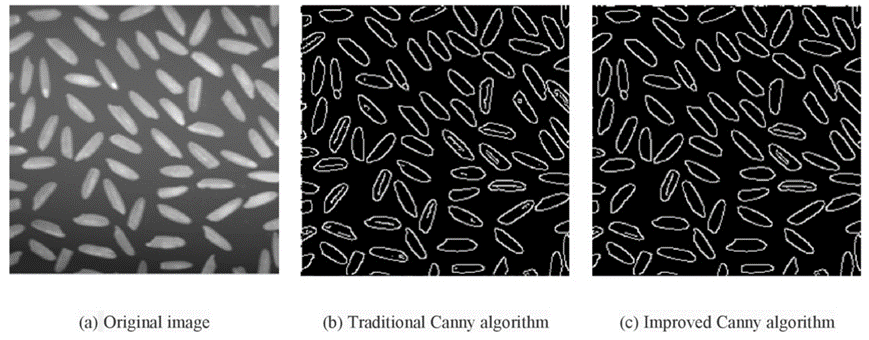
\includegraphics{2_1.png}
  \end{center}
  \caption[Poem]{หลักการทำงานของ Canny edge detection}
\end{figure}

ขั้นตอนหลักในการทำ Canny edge detection มีดังนี้:

\begin{itemize}
  \item {Gaussian Filter: เพื่อลด noise ไปจากภาพ ทำให้ไม่เกิดขอบภาพที่ไม่ต้องการ}
  \item {Prewitt หรือ Sobel edge detector: หา Edge strength และ Edge orientation}
  \item {Edge orientation Substituted: เปลี่ยนค่า orientation ของ edge ให้อยู่ในช่วงที่สามารถระบุพิกัดเป็นตำแหน่งของ pixel รอบๆได้}
\end{itemize}


\begin{figure}[h!]
  \begin{center}
    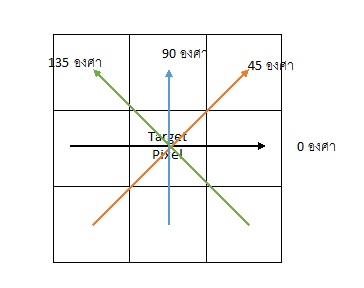
\includegraphics[height=7cm]{2_2.jpg}
  \end{center}
  \caption[Poem]{Edge orientation Substituted}
\end{figure}

\newpage
\begin{itemize}
  \item {Non-maximum Suppression}
\end{itemize}

\begin{figure}[h!]
  \begin{center}
    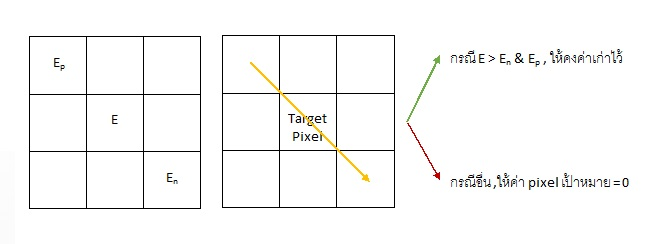
\includegraphics{2_3.jpg}
  \end{center}
  \caption[Poem]{Non-maximum Suppression}
\end{figure}

\begin{itemize}
  \item {Double threshold: เลือกค่าช่วง Edge strength ที่ต้องการแสดงไว้ และค่าที่ต่ำกว่าขอบเขตที่ระบุ ให้ค่า pixel นั้น = 0}
  \item {Hysteresis: แยกขอบออกเป็นส่วนๆ แบ่งตามตำแหน่งที่เชื่อต่อกันและความเข้ม ขอบที่มีความเข้มอ่อนจะไม่เชื่อมต่อกับขอบส่วนที่มีความเข้มสูง เราจะกำจัดส่วนนั้นทิ้งไป}
\end{itemize}

\newpage
\begin{figure}[h!]
  \begin{center}
    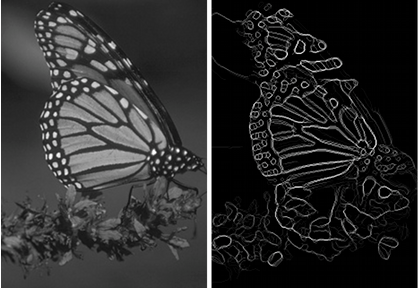
\includegraphics[height=8cm]{2_4.png}
  \end{center}
  \caption[Poem]{Hysteresis}
\end{figure}

\section{Active Contour}

เป็นเครื่องมือที่ใช้ในการตรวจจับและวาดเส้นขอบ (contour) ของวัตถุในภาพดิจิตอล โดยทั่วไปมักใช้ในการวาดเส้นขอบของวัตถุที่มีรูปร่างที่ไม่เป็นระเบียบหรือมีรูปร่างที่ซับซ้อน เช่น เครื่องตรวจจับเส้นขอบของลูกบอลในภาพถ่าย หรือการตรวจจับขอบของเซลล์ที่มีรูปทรงเป็นรูปเป็นระเบียบในภาพทางการแพทย์

\begin{figure}[h!]
  \begin{center}
    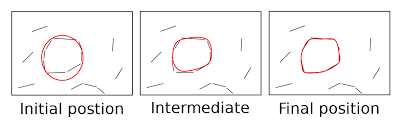
\includegraphics{2_5.png}
  \end{center}
  \caption[Poem]{หลักการทำงาน ของActive Contour}
\end{figure}

\newpage
\subsection{Active Contour : Snake Model}
เป็นโมเดลที่ใช้ใน Computer Vision สำหรับการวาดเส้นรอบวัตถุในภาพ 2 มิติ โมเดลนี้ถูกพัฒนาโดย \newline
Michael Kass, Andrew Witkin และ Demetri Terzopoulos ในปี 1987 โมเดล Snake เปรียบเสมือนเส้นยางยืดหยุ่นที่ถูกดึงดูดไปยังขอบของวัตถุในภาพ โมเดลจะใช้พลังงานสองประเภทในการดึงดูดเส้นยางไปยังขอบวัตถุ:

\begin{itemize}
  \item {พลังงานภายใน: ควบคุมความโค้งและความเรียบของเส้นยาง}
  \item {พลังงานภายนอก: ดึงดูดเส้นยางไปยังขอบของวัตถุในภาพ}
\end{itemize}

ในการนับรูปทรงต่างๆในภาพเราจะใช้  Snake Model ในการทำงานดังนี้:

\begin{enumerate}
  \item {กำหนดเส้นโค้งเริ่มต้น: เส้นโค้งเริ่มต้นสามารถกำหนดแบบสุ่ม หรือใช้ข้อมูลจากภาพ เช่น ขอบภาพ}
  \item {คำนวณพลังงาน: พลังงานจะถูกคำนวณจาก 3 องค์ประกอบ:}
  \begin{itemize}
  \item {พลังงานภายใน: วัดความเรียบของเส้นโค้ง}
  \item {พลังงานภาพ: วัดความสอดคล้องของเส้นโค้งกับภาพ}
  \item {พลังงานการเชื่อมต่อ: วัดความเชื่อมต่อของเส้นโค้ง}
  \end{itemize}
  \item {ปรับรูปร่างเส้นโค้ง: เส้นโค้งจะปรับรูปร่างของตัวเองเพื่อลดพลังงานรวม}
  \item {ทำซ้ำขั้นตอน 2 และ 3: ทำซ้ำจนกว่าเส้นโค้งจะลู่เข้า}
\end{enumerate}

\begin{itemize}
  \item {การนับรูปทรง:}
\end{itemize}

หลังจากเส้นโค้งลู่เข้าแล้ว จำนวนรูปทรงสามารถนับได้โดยการนับจำนวนเส้นโค้งที่แยกจากกัน

\begin{figure}[h!]
  \begin{center}
    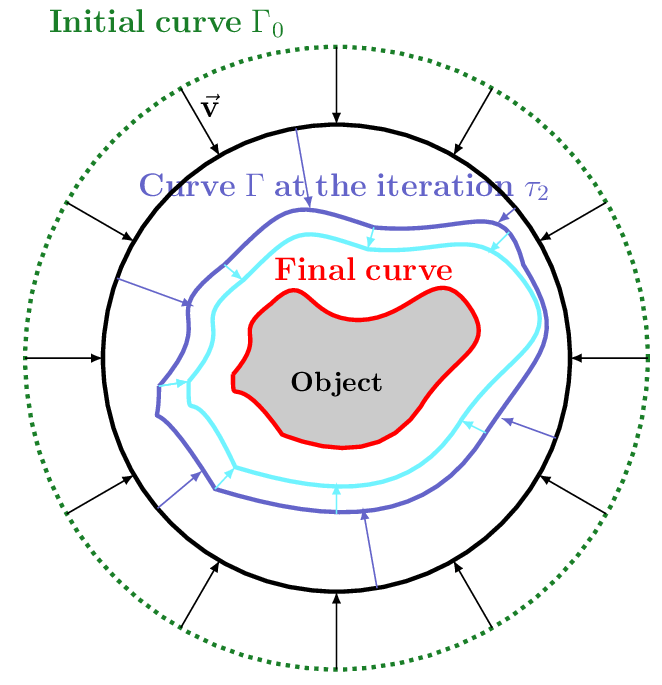
\includegraphics[height=8cm]{2_6.png}
  \end{center}
  \caption[Poem]{หลักการทำงานของ Active Contour : Snake Model}
\end{figure}

\section{\ifenglish%
Extracurricular knowledge used, applied, or integrated in this project
\else%
ความรู้นอกหลักสูตรซึ่งถูกนำมาใช้หรือบูรณาการในโครงงาน
\fi
}

\subsection{emulsion}

ระบบคอลลอยด์ (emulsion) ที่ประกอบด้วยเหลวตั้งแต่ 2 ชนิดขึ้นไป ซึ่งปกติไม่ผสมเป็นเนื้อเดียวกัน เช่น น้ำกับน้ำมัน ผสมรวมเป็นเนื้อเดียวกันได้โดยไม่แยกชั้น โดยของเหลวส่วนหนึ่งแตกตัวเป็นหยดเล็กๆ เรียกว่า วัฏภาคภายใน หรือส่วนที่กระจายตัว (internal or dispersed phase) ซึ่งจะกระจายตัวแทรกอยู่ในของเหลวอีกชนิดหนึ่ง เรียกว่า วัฏภาคภายนอก (external or continuous phase) ส่วนที่ต่อเนื่อง


อิมัลชันแบ่งเป็น 2 ประเภทหลัก คือ

\begin{itemize}
  \item {อิมัลชันชนิดน้ำมันในน้ำ (oil-in-water emulsion, O/W) มีน้ำมันเป็นวัฎภาคภายใน และน้ำเป็นวัฎภาคภายนอก เช่น น้ำนม (milk) ข้อสังเกตุ หรือวิธีทดสอบอิมัลชันประเภทนี้คือ สามารถทำให้เจือจางได้ด้วยการเติมน้ำ มีค่าการนำไฟฟ้า (electrical conductivity) สูงกว่า ผสมได้กับสีชนิดที่ละลายน้ำ (water soluble dye)}
  \item {อิมัลชันชนิดน้ำในน้ำมัน (water-in-oil emulsion, W/O) มีน้ำเป็นวัฎภาคภายใน และน้ำมันเป็นวัฎภาคภายนอก เช่น เนย (butter) มายองเนส (mayonnaise) น้ำสลัด (salad dressing) ไส้กรอก (sausage) ข้อสังเกตุ หรือวิธีทดสอบอิมัลชันประเภทนี้คือ สามารถทำให้เจือจางได้ด้วยการเติมน้ำมัน มีค่าการนำไฟฟ้า (electrical conductivity) ต่ำกว่า ผสมได้กับสีชนิดที่ละลายน้ำมัน (oil soluble dye)}
  \end{itemize}\

  \begin{figure}[h!]
    \begin{center}
      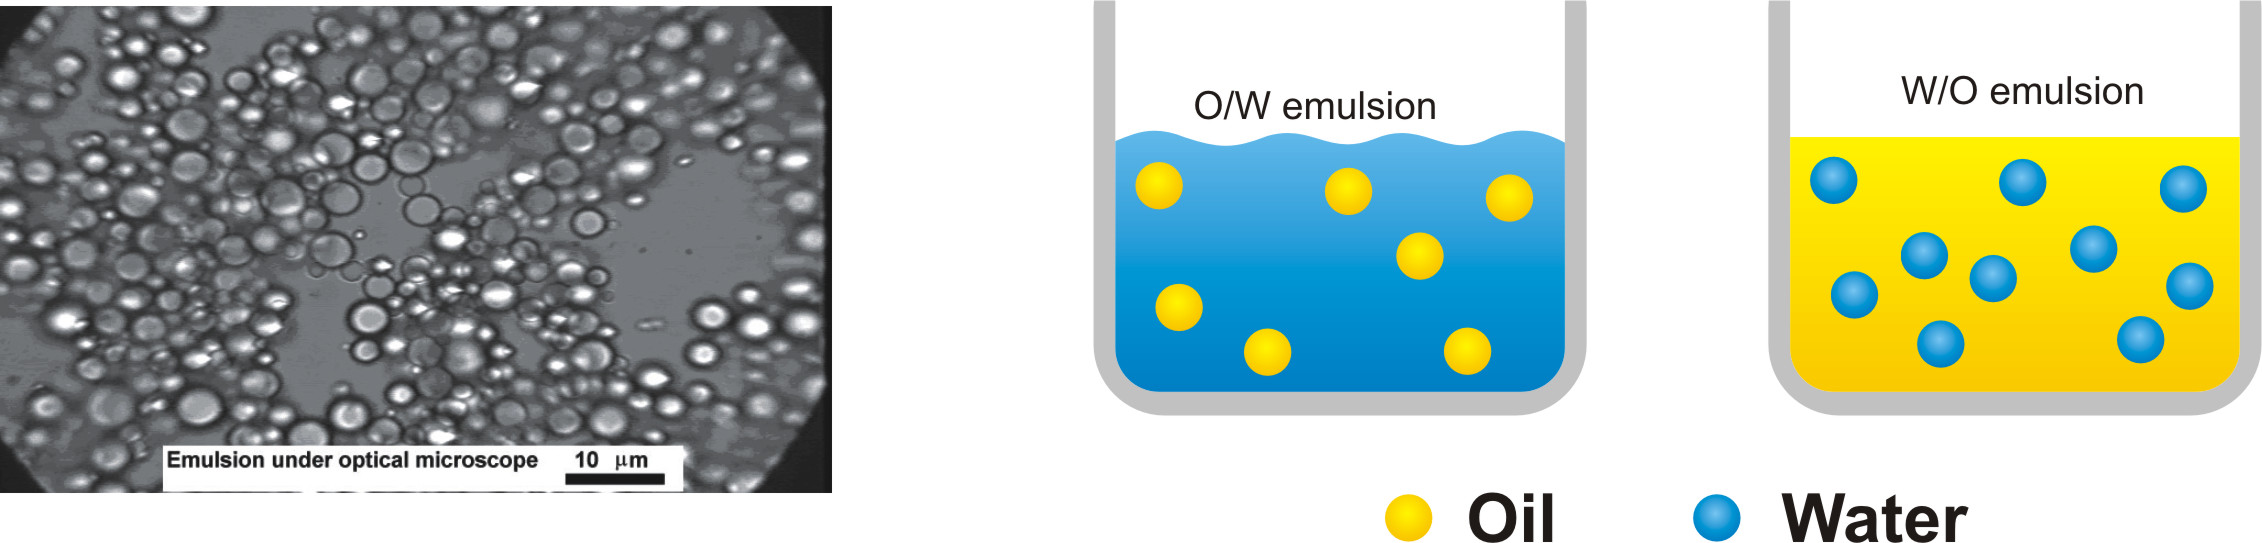
\includegraphics[width=\textwidth]{2_7.jpg}
    \end{center}
    \caption[Poem]{emulsion}
  \end{figure}
